\documentclass[
    % draft,                             % 草稿模式
    aspectratio=169,                   % 使用 16:9 比例
]{beamer}
\mode<presentation>
\usetheme[
    % navigation=subsections,            % 使用子章节进度显示
    % lang=en,                           % 使用英文
    % cjk=true,                          % 使用CJK而不是ctex
    color=red,                         % 使用红色主题
    % pattern=all,                        % 使用全图案装饰
    % gbt=bibtex,                        % 使用 gbt (使用 bibtex 编译)
]{sjtubeamermin}
\usecolortheme[]{beaver}                 % 使用其他颜色主题
\addbibresource{ref.bib}               % gbt!=bibtex

\begin{document}
    % \institute[School of Electrical Engineering]{数学科学学院}   % 组织
    \institute[Department of Automation]{自动化系}   % 组织
    \logo{
        
\includegraphics{cnlogored.pdf}  % 重定义 logo
    }
    \titlegraphic{                         % 标题图像
        \begin{stampbox}
            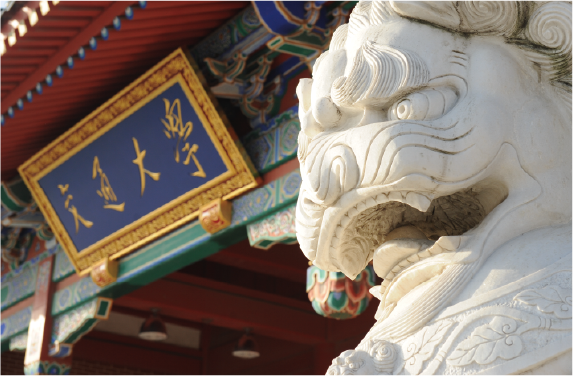
\includegraphics[width=0.3\textwidth]{head.png}
        \end{stampbox}
    }
    \title{Blockchain and Internet of Things 区块链和物联网}  % 标题
    \subtitle{Access Control Management}         % 副标题
    \author{Pedro Hernández Rubio}                  % 作者
    \date{\today}                          % 日期  
    \maketitle                             % 创建标题页

\part{第一部分 Blockchain technologies applied to IoT architecture}

% 使用节目录
\AtBeginSection[]{
    \begin{frame}
        % \tableofcontents[currentsection]           % 传统节目录             
        \sectionpage                   % 节页
    \end{frame}
}

% 使用小节目录
% \AtBeginSubsection[]{                  % 在每小节开始
%     \begin{frame}
%         \tableofcontents[currentsection,currentsubsection]             % 传统小节目录             
%         \subsectionpage                % 小节页
%     \end{frame}
% }

\section{第 1 节 Blockchain applied to IoT}

\subsection{第 1 小节 Integrating Blockchain and IoT}

    \begin{frame}
        \frametitle{Integrating Blockchain and IoT}

        \paragraph{Goal} Research the use of \alert{Blockchain technologies} and \alert{P2P storage systems} for IoT systems management.

        \begin{itemize}
            \item \alert{Decentralized}: IoT devices data are not required to be sent to centralized services (default trust): data can be stored securely on the peers in the network, anb blockchain assure its authenticity and control authorized accesses.
            \item \alert{Private-by-design IoT}: providing privacy, robust systems and no single point of failure.
        \end{itemize}

        \begin{block}{Security}
            All operations involving IoT devices in the network can be registered and authenticated in the blockchain: data creation, data modification or data deletion. IoT devices security could be drammatically enhanced
        \end{block}

    \end{frame}

\subsection{第 2 小节 Uses cases}

    \begin{frame}
        \frametitle{Use cases}

        \begin{block}{Beyond criptocurrencies}
            Paradigm of decentralizing services that so far have depend exclusively of centralized trusting authorities. But possible applications are endless.
        \end{block}

        \paragraph{Research} Several use cases were found on the literature:

        \begin{itemize}
            \item \alert{Data store management}: data collected by IoT devices can be stored in a blockchain as a single point of truth.\cite{sia}
            \item \alert{Authentication service}: by public key cryptography, all IoT devices can be securely identified in order to communicate safely among them.\cite{Axon2015PrivacyawarenessIB}
            \item \alert{Exchanging data}: data collected by devices on one specific network can be traded (or exchanged) according to common establised policies.
        \end{itemize}

    \end{frame}

\subsection{第 3 小节 Blockchain factors for IoT}

    \begin{frame}
        \frametitle{Blockchain factors for IoT (I)}

        \begin{block}{Integrity}
            IoT applications can be securely developed on top of stable blockchain networks, by building a layered architecture with thin clients.\cite{Ali2016BlockstackDA} Thus, consensus protocols and large enough nodes community make possible attacks mostly unfeasible
        \end{block}
        \begin{block}{Anonimity}
            As most of blockchain networs are public, full anonimity is not achieved (IoT devices can still be linked to their respective owners) -> \alert{pseudonimity}
            Methods for not associating public keys to IoT devices' IDs are being investigated.\cite{Axon2015PrivacyawarenessIB}
        \end{block}

    \end{frame}

    \begin{frame}
        \frametitle{Blockchain factors for IoT (II)}

        \begin{block}{Adaptability}
            Poor scalability and low throughput of transactions are the biggest issues related to IoT systems. An acceptable trade-off between security and scalability must be determined.\cite{conoscenti}
        \end{block}

        Mitigations:
        \begin{itemize}
            \item \alert{Layered architecture}: IoT applications built on top of scalable blockchain network.
            \item \alert{Data storage}: allowing thin clients to delegate some data in the blockchain, as many IoT devices have limited resources.\cite{Axon2015PrivacyawarenessIB}
        \end{itemize}

    \end{frame}

    % \begin{frame}
    %     \frametitle{标题}
    %     \framesubtitle{子标题}

    %     \begin{equation}
    %         x^2+2x+1=(x+1)^2
    %     \end{equation}
        
    % \end{frame}

\section{第 2 节 IoT Access Control}

\subsection{第 1 小节 Decentralized Access Control}

    \begin{frame}
        \frametitle{Decentralized Access Control}
        
        \paragraph{Goal} Research decentralized access control solutions for IoT systems management.\cite{ouaddah}

        \begin{itemize}
            \item \alert{DOAuth}: IoT devices data are not required to be sent to centralized services (default trust): data can be stored securely on the peers in the network, anb blockchain assure its authenticity and control authorized accesses.
            \item \alert{FairAccess}: providing privacy, robust systems and no single point of failure.
        \end{itemize}

        \begin{block}{Scalability issue}
            All operations involving IoT devices in the network can be registered and authenticated in the blockchain: data creation, data modification or data deletion. IoT devices security could be drammatically enhanced.
        \end{block}
    \end{frame}

\subsection{第 2 小节 Security issues}

    \begin{frame}
        \frametitle{Current optimal solution}
        
        \begin{block}{Scalable Access Management}
            Because of scalability issues, a feasible solution involves a layered architecture with access control policies stored as smart contracts.\cite{novo}
        \end{block}

        \paragraph{Decision} Main advantages of this access control in IoT:

        \begin{Main}
            \item \alert{Mobility}: 
            \item \alert{Accessibility}: 
            \item \alert{Concurrency}: 
            \item \alert{Lightweight}: 
            \item \alert{Scalability}: 
            \item \alert{Transparency}: 
        \end{itemize}
    \end{frame}

\subsection{第 3 小节 IoT architecture (I)}

    \begin{frame}
        \frametitle{IoT architecture (I)}

        \begin{block}{Smart contract}
            Access control management information is stored in the blockchain layer.\cite{novo}
        \end{block}
        
        \begin{figure}
            \centering
            \begin{stampbox}
                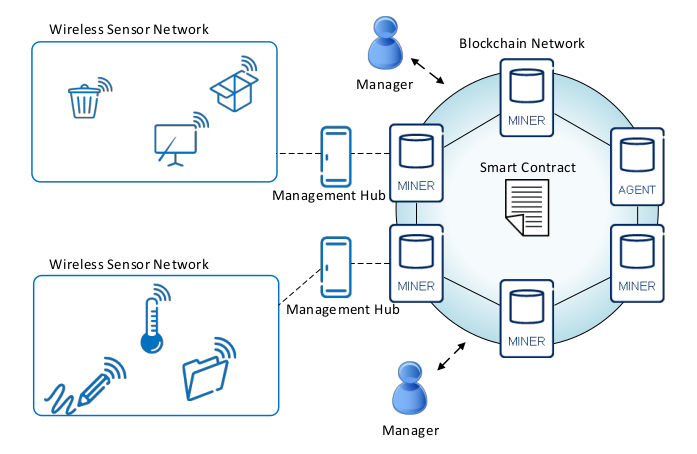
\includegraphics[height=0.6\textheight]{iot-architecture.png}
            \end{stampbox}
            \caption{Decentralized Access Control Architecture}
        \end{figure}
    \end{frame}

\subsection{第 4 小节 IoT architecture (II)}

    \begin{frame}
        \frametitle{IoT architecture (II)}

        \paragraph{Architecture} Components classification:

        \begin{block}{Outside blockchain network}
            \begin{itemize}
                \item \alert{Wireless sensor networks}: IoT devices 
                \item \alert{Management hubs}:
            \end{itemize}
        \end{block}

        \begin{block}{Inside blockchain network}
            \begin{itemize}
            \item \alert{Managers}: 
            \item \alert{Agent node}:
            \item \alert{Smart contract}: 
            \item \alert{Blockchain network}: 
            \end{itemize}
        \end{block}
    \end{frame}

%     \begin{frame}[fragile]          % 注意添加 fragile 标记
%         \frametitle{代码块}
%         % 代码块参数:语言,标题
%         % 请减少代码初始的缩进
%         \begin{codeblock}[language=c++]{C++代码}
% #include<iostream>

% int main(){
%     // Console Output
%     std::cout << "Hello, SJTU!" << std::endl;
%     return 0;
% }
%         \end{codeblock}
%     \end{frame}

%     \begin{frame}
%         \frametitle{图}
%         \begin{figure}
%             \centering
%             \begin{stampbox}
%                 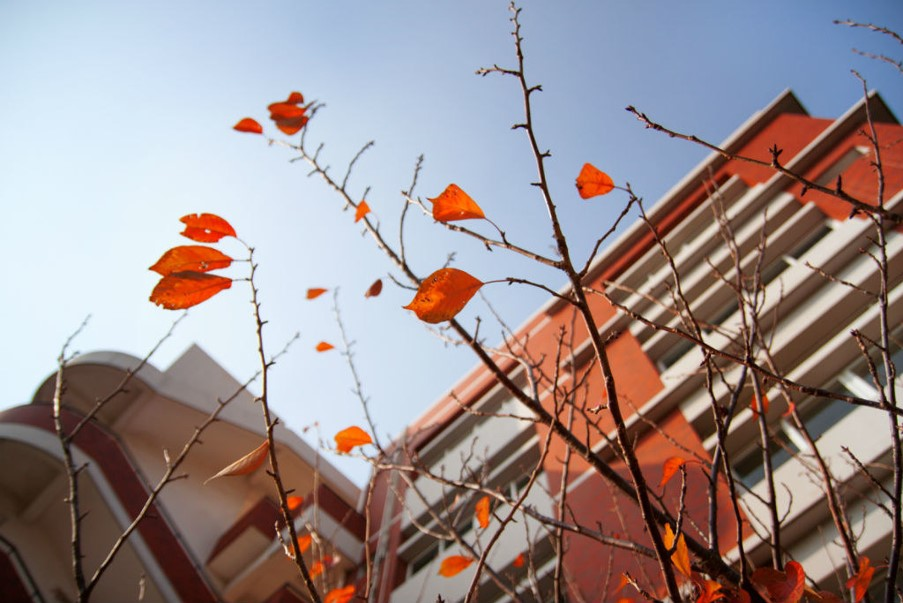
\includegraphics[height=0.3\textheight]{plant.jpg}
%             \end{stampbox}
%             \caption{图片标题\cite{viman}}
%         \end{figure}
%     \end{frame}

%     \begin{frame}
%         \frametitle{表与统计图}
%         \begin{multicols}{2}
%         \begin{table}
%             \caption{表格标题\cite{pgfplotstableman}}
%             \pgfplotstabletypeset[
%                 columns/Quick/.style={dec sep align},
%                 columns/Cocktail/.style={dec sep align},
%                 column type=r,
%                 % fixed zerofill,
%             ]{test.csv}
%         \end{table}
        
%         \begin{figure}
%             % !TeX root = ../main.tex
% Made with PGFPlotsEdt:
% https://logcreative.github.io/PGFPlotsEdt/
\begin{tikzpicture}
    \begin{axis}[
    height=0.45*\the\paperheight,
    xlabel={$n$},
    ylabel={Average Steps},
    ymin={0},
    xmax={9},
    xmin={1},
    legend style={at={(0.5,1.05)},anchor=south},
    legend columns=2,
    grid,
    minor tick num=1]
     \pgfplotstableread {test.csv}{\foo};           % read table
     \addplot+ [only marks,mark options={scale=0.8}] table[y=Quick] {\foo};
     \addplot+ [only marks,mark options={scale=0.8}] table[y=Cocktail] {\foo};
     \pgfplotsset{cycle list shift=-2};                 % start the cycle list from beginning
     \addplot+ [no markers,domain=1:9,] {1.502*x*ln(x)};
     \addplot+ [no markers,domain=1:9,] {0.4453*x*x-0.1365*x-0.473};
     \legend{Quick,Cocktail,}                           % only mark the first two series
    \end{axis}
\end{tikzpicture}
%             \caption{统计图标题\cite{pgfplotsman}}
%         \end{figure}
%         \end{multicols}
%     \end{frame}


% gbt=bibtex
\part{References 参考文献}
    \begin{frame}[allowframebreaks]
        \printbibliography[title=References 参考文献]    % gbt!=bibtex
        % \bibliography{ref.bib}             % gbt=bibtex
    \end{frame}

    \makebottom     % 创建尾页  % 非标准命令

\end{document}